\section{ANÁLISE DE CARGA DA INSTALAÇÃO}

\hspace*{0.8cm} Este capítulo aborda a análise do das características de consumo. O diagrama esquemático deste sistema está exposto na  Figura \ref{fig:dia}. Deste diagrama, tem-se os eletrodos, que estão conectados no paciente; o cir\-cuito de aquisição para tratar e acomodar o sinal enquanto o MCP3008 é utilizando como conversor analógico/digital e se conecta com o Raspberry Pi 3 através da porta SPI. Ambos estão configurados para transmitir o sinal ECG. O sistema é iniciado com o pedido realizado pelo usuário, utilizando a arquitetura cliente-servidor presente nos computadores. Internamente o cliente
faz a requisição ao servidor presente no Raspberry Pi 3 e o interpreta, utilizando a rede Wi-Fi como meio de comunicação, realizando a leitura de dados da porta do MCP3008, a qual está conectada com o circuito de aquisição e por fim, o cliente recebe as amostras, fornecida pelo o servidor. \textcolor{red}{há extra "espaços"...verifique isso....acho que vc poderia quebrar esse para em dois e explicar um pouco melhor}


\begin{figure}[H]
\begin{center}
			\caption{Diagrama Esquemático do Sistema Proposto}
			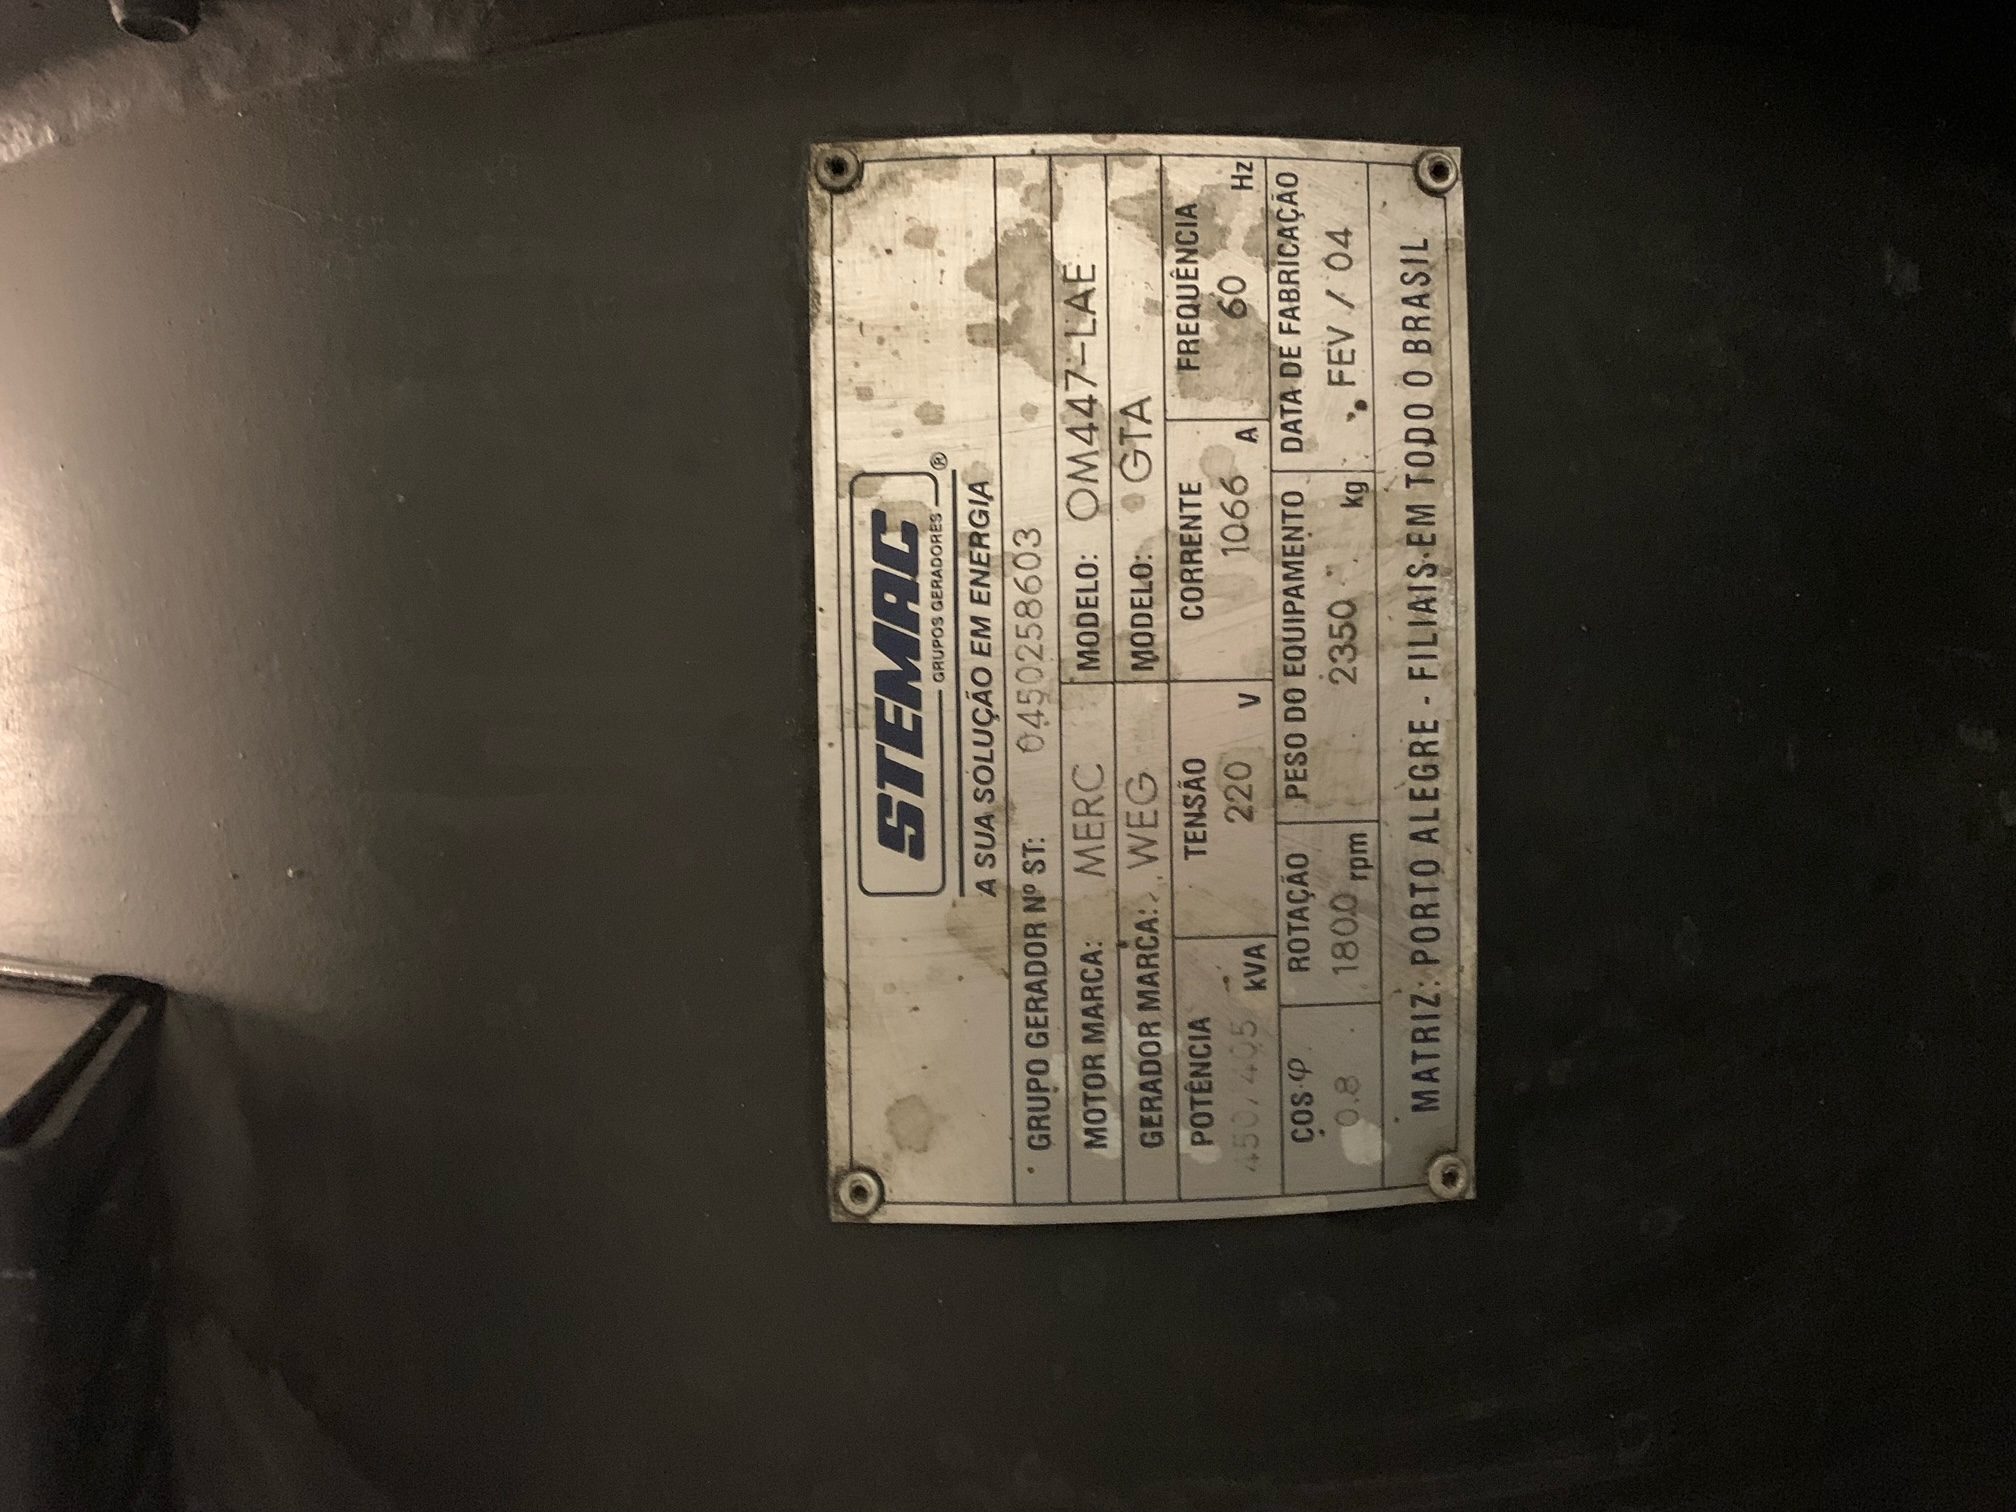
\includegraphics[width=.8\textwidth]{Figuras/info_gerador_450.jpeg}
            \vspace*{\fill} 
            \begin{quote} 
            \centering 
           Fonte: {Elaborada pela autora}
            \end{quote}
            \vspace*{\fill}
			\label{fig:dia}

\end{center}
\end{figure}



\subsection{DESENVOLVIMENTO DO HARDWARE}
\hspace*{0.8cm}Após a etapa de definição e aquisição de componentes que fazem parte da configuração do hardware, procedeu-se a implementação do circuito eletrônico em um protoboard, sendo que inicialmente foram realizados testes nos componentes eletrônicos. O primeiro teste consistiu na verificação dos sinais ECG utilizando a placa ECG AD8232, a qual foi alimentada com a tensão de 3,3V e utilizou o  pino GND para aterramento do sinal. Utilizou-se os pinos RA, LA e RL do simulador de sinais vitais HS-15 no modo ECG, conectado nos pinos RA, LA e RL da placa AD8232 com o intuito de analisar a forma de onda característica do sinal ECG, com o manuseio da ponta de prova do osciloscópio e assim analisar o sinal na tela do equipamento. \textcolor{red}{verifique os "espaços" novemente}